\documentclass[11pt,a4paper]{article}
\usepackage[utf8]{inputenc}
\usepackage[english]{babel}
\usepackage[margin=2.5cm]{geometry}
\usepackage{booktabs,graphicx,amsmath,microtype,array,float}
\usepackage[colorlinks=true,linkcolor=black,citecolor=black,urlcolor=blue!45!black]{hyperref}
\usepackage{xcolor}
\setlength{\parindent}{1.2em}
\setlength{\parskip}{0.25em}
\renewcommand{\arraystretch}{1.12}
\hypersetup{pdftitle={Women among agricultural producers in Peru, 2014--2025: recorded status and service access in 2025},pdfauthor={Renato Quispe Vargas and Kemelly Shanell Ilaquita Pariapaza}}

\begin{document}
\begin{center}
{\LARGE\bfseries Women among agricultural producers in Peru, 2014--2025:\par}
\vspace{2mm}
{\large Recorded producer status and service access in 2025\par}
\vspace{5mm}
{\normalsize Renato Quispe Vargas \quad and \quad Kemelly Shanell Ilaquita Pariapaza\par}
\end{center}

\begin{abstract}
\noindent\textbf{Background:} The sex of a survey-identified agricultural producer describes who is recorded as managing a farm unit, but does not directly measure women's labor, land rights, or autonomy. We examined this measure across eleven rounds of Peru's National Agricultural Survey (ENA) and, in 2025, compared access to agricultural services and finance.

\noindent\textbf{Methods:} We analysed 330,134 eligible producer records from 2014--2019 and 2021--2025 using annual expansion weights and survey-weighted models. Historical confidence intervals use an explicit round-by-department design approximation. We estimated associations separately in 2014--2022 and 2023--2025 and evaluated a model trained through 2024 on 2025. For the 2025 round, four official modules were linked one-to-one for 38,449 producers; access outcomes were analysed using the recorded sampling strata.

\noindent\textbf{Results:} The weighted female share was 28.99\% (approximate 95\% CI 28.09--29.89) in 2014, 33.35\% (32.44--34.26) in 2022, and 31.18\% (29.35--33.01) in 2025. The primary-schooling versus no/initial-schooling adjusted odds ratio was 0.219 (95\% CI 0.206--0.233), with the same direction in both survey eras. Out-of-time discrimination was modest (weighted AUC 0.615). In 2025, training was reported by 5.28\% of female and 8.37\% of male producers; credit application by 8.37\% and 11.65\%, respectively. Fully adjusted female-minus-male differences were $-2.29$ (95\% CI $-4.93$ to 0.36) and $-1.27$ ($-3.38$ to 0.85) percentage points.

\noindent\textbf{Conclusion:} The eleven-round series describes changing recorded producer shares across survey-specific populations, while the 2025 modules show contemporaneous access gaps. Survey-frame changes, incomplete historical provenance, and unmeasured determinants prevent strictly like-for-like temporal or causal interpretations.
\end{abstract}

\noindent\textbf{Keywords:} Peru; Encuesta Nacional Agropecuaria; women agricultural producers; repeated cross-sections; extension services; credit; complex surveys; reproducibility.

\section{Introduction}
The expression ``feminization of agriculture'' has been used for women's farm labor, their identification as farm managers, and their control of agricultural resources. These outcomes are related but not interchangeable. A larger female share of recorded producers may reflect changes in who operates a unit, in survey coverage, or in household designation; it cannot establish increased autonomy or hardship on its own. Empowerment also involves agency and achievements, dimensions that a producer-sex field does not measure \cite{kabeer1999}. Comparative work has cautioned against treating women's agricultural roles as a single phenomenon or inferring mechanisms from a headship indicator \cite{deere2005,doss2018,kawarazuka2022,leder2022}. The Food and Agriculture Organization likewise distinguishes participation from access to assets, services, and decision-making \cite{fao2023}. Research on Latin American land ownership further shows why a recorded farm operator cannot automatically be treated as the legal owner \cite{deereleon2003}.

Peru's ENA offers repeated national measurements of the person identified as an agricultural producer. Official ENA reporting indicates that women represented about one third of producers in recent rounds \cite{inei2022,ineigender2025,inei2025results}. Studies in Peru have examined gender gaps in agricultural assets, differences among Sierra potato farmers, land ownership and food security, joint titling, and decisions about value-chain participation \cite{delpozo2016,patel2018,schling2024,wiig2013,tobin2022}. Those studies address outcomes and populations that differ from the sex of the ENA-identified producer. The agricultural policy context also differs sharply between coastal export-oriented production and many smaller farms \cite{oecd2026}. A pooled ENA series therefore warrants care: the survey frame and selection procedures changed, and the available historical analytical file does not preserve every official design variable. The question is narrower than whether Peruvian agriculture has undergone a causal transition toward female control.

We address four descriptive and associational objectives. First, we estimate the weighted female share in each available ENA round from 2014 through 2025. Second, we describe how recorded producer sex varies by age, schooling, and natural region and estimate adjusted associations. Third, we assess whether the direction of key associations persists across survey eras and whether a model estimated before 2025 transports to that round. Fourth, using additional modules available for 2025, we compare training, technical assistance, credit application, savings accounts, and receipt of requested credit among female and male producers. The historical series and the 2025 access analysis have different estimands and variance designs; only the producer-sex measure is followed across rounds. None of these objectives identifies mechanisms based on migration, land title, credit decisions, or empowerment.

\section{Data and methods}
\subsection{Study design and source files}
This is an analysis of repeated cross-sectional ENA records, not a longitudinal study of identified people. Eleven rounds are included: 2014--2019 and 2021--2025; the ENA was not conducted in 2020 during the COVID-19 emergency \cite{ineiods2025}. The historical input is a project-supplied consolidated SPSS file for 2014--2024, and the final round comes from the official 2025 Chapter 1100 file available through the INEI Microdata Portal \cite{ineiportal}. The historical consolidation procedure was not supplied, a provenance limitation described below. Reporting of eligibility, variables, missingness, and design limitations was informed by applicable STROBE recommendations for observational studies \cite{strobe2007}.

The survey target changed across the period. Documentation for 2018/2019 describes a frame of small and medium producers up to 50 hectares and a two-stage area design \cite{inei2018,inei2019}; the 2023 manual describes a frame up to 999 hectares, while the 2025 technical sheet describes departmental samples of segments selected in one stage \cite{inei2023,inei2025}. The 2025 area-frame population comprises units with agricultural area conducted by natural persons and excludes peasant and Indigenous communities; a knowledgeable adult other than the producer can answer the interview \cite{inei2025}. Annual estimates therefore refer to their respective survey populations. Connecting points in a figure does not make them estimates of a constant cohort or a harmonized target population. The 2019 documentation also describes panel and newly sampled units; repeated units across rounds may violate an independence approximation \cite{inei2019}.

\subsection{Participants, variables, and missing data}
The analytical unit is a record with producer identifier P1102 equal to 1. We retained completed interviews (RESFIN=1), valid sex codes (P1103: 1 male, 2 female), age 15--100 years (P1104\_A), schooling codes 1--10 (P1105), natural-region codes 1--3, a positive expansion weight, and a nonmissing segment identifier. The binary outcome is female producer status. Schooling codes were grouped as no schooling/initial (1--2), primary (3--4), secondary (5--6), and higher (7--10), following the 2025 data dictionary \cite{inei2025dict}. These levels do not identify literacy. Natural region was coded Coast, Sierra, or Selva.

Of 330,338 producer records, 200 had incomplete interviews. Four completed 2014 records had education code 99 and were excluded rather than silently assigned to a schooling level. All 330,134 retained records had valid positive weights and segment identifiers; no covariate values were imputed. We used every eligible record, without a separate power-based sample-size calculation. Table~\ref{tab:annual} gives annual sample sizes. The sum of the expansion weights is 25.30 million \emph{producer-rounds}, not a count of unique persons or a single-year population.

\subsection{Estimands and survey-weighted analysis}
For each round, the descriptive estimand is the weighted proportion of retained producer records coded female. Annual weights are FACTOR through 2022 and FACTOR\_PRODUCTOR from 2023. Historical primary sampling units were reconstructed from CONGLOMERADO; later rounds use NSEGM. We keyed units by round, department, and segment, and specified round-by-department analytical strata. The resulting design has 42,327 observed clusters, 273 strata, and 42,054 design degrees of freedom. Taylor-linearized standard errors were calculated with the R \texttt{survey} package \cite{lumley2004}. These strata are an approximation because the consolidated historical file lacks complete official stratification identifiers. Thus the reported confidence intervals are conditional on this working design and do not reproduce official INEI variance estimates.

The adjusted association model is
\begin{equation}\label{eq:logit}
\operatorname{logit}\{\Pr(Y_i=1\mid X_i)\}
=\beta_0+\beta_1\mathrm{age}_i+\beta_2(\mathrm{age}_i/10)^2
+\boldsymbol\gamma^{\mathsf T}\mathrm{education}_i
+\boldsymbol\delta^{\mathsf T}\mathrm{region}_i
+\boldsymbol\tau^{\mathsf T}\mathrm{round}_i,
\end{equation}
where $Y_i=1$ is a female producer record. The reference levels are no/initial schooling, Coast, and 2014. A quasibinomial survey-weighted logit was fitted. Odds ratios compare conditional odds at fixed modeled covariates; they are neither probability differences nor effects of changing schooling or residence. We did not use round coefficients to estimate a causal time effect.

For sensitivity to the major frame change, the same specification was fitted separately for 2014--2022 and 2023--2025, with round indicators within each era. To provide an absolute-scale interpretation, we predicted from the pooled model over the weighted 2025 covariate distribution while setting one schooling or region level at a time. Approximate delta-method intervals use the model coefficient covariance matrix and condition on that covariate distribution. These standardized predictions are associational scenarios.

For out-of-time assessment, we fitted a separate model without round indicators using 2014--2024 data and evaluated it on 2025. We report weighted AUC for discrimination, Brier score for overall probability error, and the weighted mean predicted and observed female shares for calibration in the large; a weighted decile plot displays local calibration \cite{steyerberg2010}. The Brier comparator is a constant prediction equal to the weighted female share in the training rounds. These performance measures describe this particular temporal split across survey eras, not prospective individual validity. Calculations used R 4.5.2 and \texttt{survey} 4.5; software versions are recorded in the replication archive.

\subsection{Additional 2025 service-access analysis}
To contextualize the endpoint of the eleven-round series, we linked the official 2025 modules for operated agricultural area (Chapter 100A), extension services (Chapter 700), financial services (Chapter 900), and producer characteristics (Chapter 1100). The key comprised year, department, province, district, segment, and agricultural unit. All 38,449 producer records had a unique one-to-one match across the four modules. This analysis uses the same producer definition as the historical series, but no comparable all-round service file was constructed.

Chapter 700 records training (P701) and technical assistance (P704) over the previous three years. Chapter 900 records a credit application (P901), receipt of requested credit (P902), and a savings account (P907) over the previous 12 months. Application and account rates use all producers as denominator; credit receipt uses applicants only. Positive responses have code 1. Sex is the binary survey code P1103, not a measure of gender identity. Descriptive female-minus-male prevalence differences use FACTOR\_PRODUCTOR, department-by-segment primary sampling units, and the recorded 2025 sampling stratum. The 2025 file has 9,125 observed segments and 4,322 recorded strata, of which 3,412 contain one observed segment. Taylor-linearized intervals use \texttt{survey.lonely.psu="adjust"} and domain adjustment; no finite-population correction was available. These intervals and the historical round-by-department intervals are distinct analytical approximations, not official INEI intervals \cite{lumley2004,surveydocs}.

For each of four access outcomes, we fitted a survey-weighted quasibinomial model with sex, age, age squared, schooling, and natural region. A second specification added log(1 + operated hectares) and a missing-area indicator; 19 area observations were missing. We standardized sex-specific predictions over the common weighted 2025 covariate distribution and report their difference in percentage points. Approximate delta-method intervals condition on that distribution. Receipt of requested credit was modelled separately among applicants, including a sensitivity specification with department fixed effects and another using department rather than the recorded sampling stratum. Models describe associations; adjustment for operated area may condition on part of a pathway linking unequal resources to service access. No causal or discrimination interpretation is assigned to the selected-applicant comparison.

\section{Results}
\subsection{Annual distribution and sample flow}
The weighted female share was 28.99\% in 2014 and reached 33.35\% in 2022; it was 31.97\% in 2023, 31.46\% in 2024, and 31.18\% in 2025 (Table~\ref{tab:annual}, Figure~\ref{fig:trend}). All 2014--2023 estimates agree to one decimal place with the INEI's retrospective table, and the 2024 and 2025 estimates agree with published figures of 31.5\% and 31.2\% \cite{inei2023results,ineigender2025,inei2025results}. This external agreement checks the annual point estimates, not the analytical confidence intervals. The measured sequence is not monotonic. In particular, the discontinuity in survey coverage at 2023 prevents reading the entire series as a like-for-like change in the same population.

\begin{table}[htbp]
\centering\small
\caption{Producer records and survey-weighted female share by ENA round.}
\label{tab:annual}
\begin{tabular}{rrrrl}
\toprule
Round & Identified & Complete & Analysed & Female share, \% (approx. 95\% CI) \\
\midrule
2014 & 26,177 & 26,119 & 26,115 & 28.99 (28.09--29.89) \\
2015 & 26,874 & 26,817 & 26,817 & 29.38 (28.45--30.32) \\
2016 & 28,158 & 28,112 & 28,112 & 29.60 (28.73--30.46) \\
2017 & 28,170 & 28,136 & 28,136 & 29.81 (28.94--30.68) \\
2018 & 28,110 & 28,110 & 28,110 & 30.03 (29.16--30.89) \\
2019 & 28,038 & 28,037 & 28,037 & 30.78 (29.91--31.64) \\
2021 & 28,030 & 28,029 & 28,029 & 31.21 (30.31--32.11) \\
2022 & 30,292 & 30,289 & 30,289 & 33.35 (32.44--34.26) \\
2023 & 30,526 & 30,526 & 30,526 & 31.97 (29.92--34.01) \\
2024 & 37,514 & 37,514 & 37,514 & 31.46 (29.37--33.55) \\
2025 & 38,449 & 38,449 & 38,449 & 31.18 (29.35--33.01) \\
\midrule
Total & 330,338 & 330,138 & 330,134 & --- \\
\bottomrule
\end{tabular}
\begin{minipage}{0.94\textwidth}\footnotesize\vspace{2mm}
Four 2014 records with P1105=99 were excluded after the completed-interview filter. Intervals use the analytical round-by-department strata and should not be treated as official INEI intervals. The 2020 round is absent.
\end{minipage}
\end{table}

\begin{figure}[htbp]
\centering
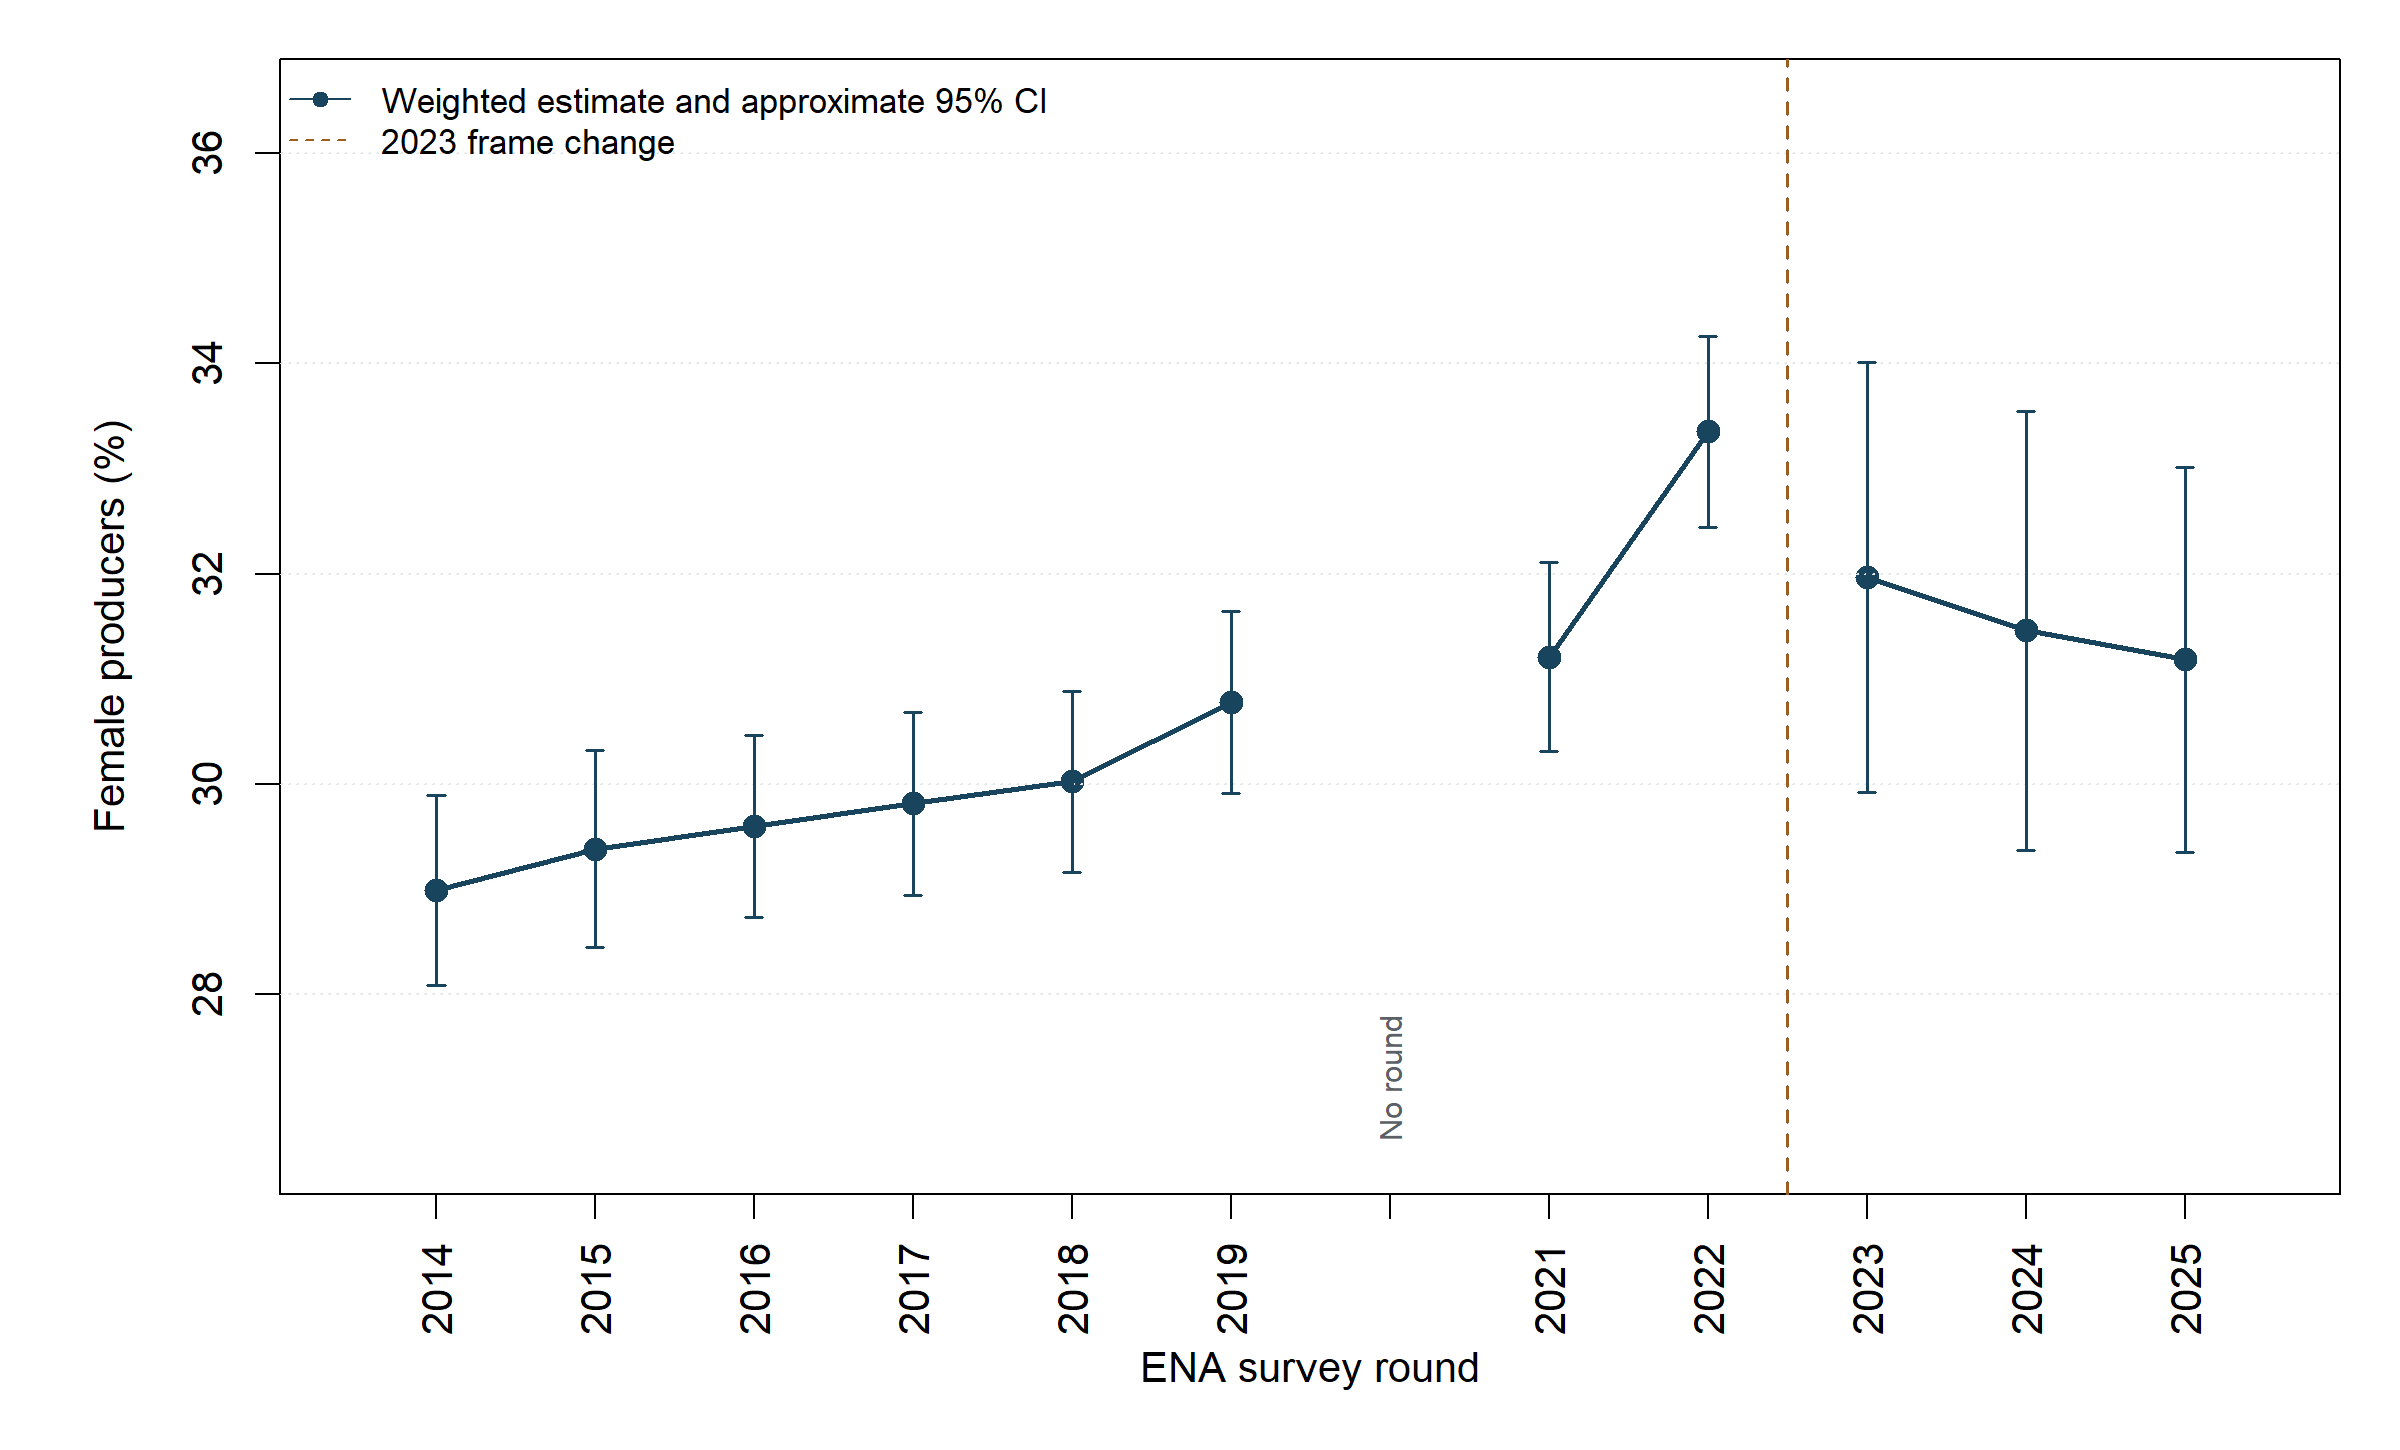
\includegraphics[width=0.93\textwidth]{figure1_female_share_ci.png}
\caption{Female share among survey-identified agricultural producers by round. Points and intervals are weighted estimates and approximate 95\% confidence intervals under the analytical design. Lines connect rounds within a survey era for visual orientation; no causal or constant-population trend is implied. The dashed line marks the 2023 frame change.}
\label{fig:trend}
\end{figure}

\subsection{Age, schooling, and region}
Across pooled producer-rounds, the weighted mean age was 53.71 years: 54.62 among women and 53.30 among men. Among female producers, 27.47\% were aged 65 years or older, compared with 24.59\% of male producers; 4.69\% of all producers were younger than 30. These are pooled record-level descriptions, not 2025-only demographic estimates.

The no/initial-schooling group had the highest female share (62.35\%, approximate 95\% CI 61.20--63.51), while women accounted for 28.47\% of the primary-schooling group and 23.09\% of the secondary-schooling group (Table~\ref{tab:groups}, Figure~\ref{fig:subgroups}). The Sierra accounted for 68.02\% of pooled weighted producer-rounds and had a female share of 34.69\% (34.14--35.23), compared with 25.37\% (24.70--26.04) on the Coast and 20.04\% (19.40--20.68) in the Selva. The percentages within a group describe its sex composition; they are not the percentages of women with that schooling or region.

\begin{table}[htbp]
\centering\small
\caption{Composition of pooled producer-rounds by schooling and natural region.}
\label{tab:groups}
\begin{tabular}{lrrl}
\toprule
Group & Records & Weighted share, \% & Female within group, \% (approx. 95\% CI) \\
\midrule
No/initial schooling & 31,956 & 11.86 & 62.35 (61.20--63.51) \\
Primary & 160,020 & 51.82 & 28.47 (27.94--29.01) \\
Secondary & 104,541 & 28.27 & 23.09 (22.44--23.74) \\
Higher & 33,617 & 8.05 & 25.51 (24.46--26.56) \\
\midrule
Coast & 69,823 & 13.64 & 25.37 (24.70--26.04) \\
Sierra & 192,990 & 68.02 & 34.69 (34.14--35.23) \\
Selva & 67,321 & 18.34 & 20.04 (19.40--20.68) \\
\bottomrule
\end{tabular}
\begin{minipage}{0.94\textwidth}\footnotesize\vspace{2mm}
Weighted shares sum within schooling or region, not across both panels. Intervals use the same approximate design as Table~\ref{tab:annual}.
\end{minipage}
\end{table}

\begin{figure}[htbp]
\centering
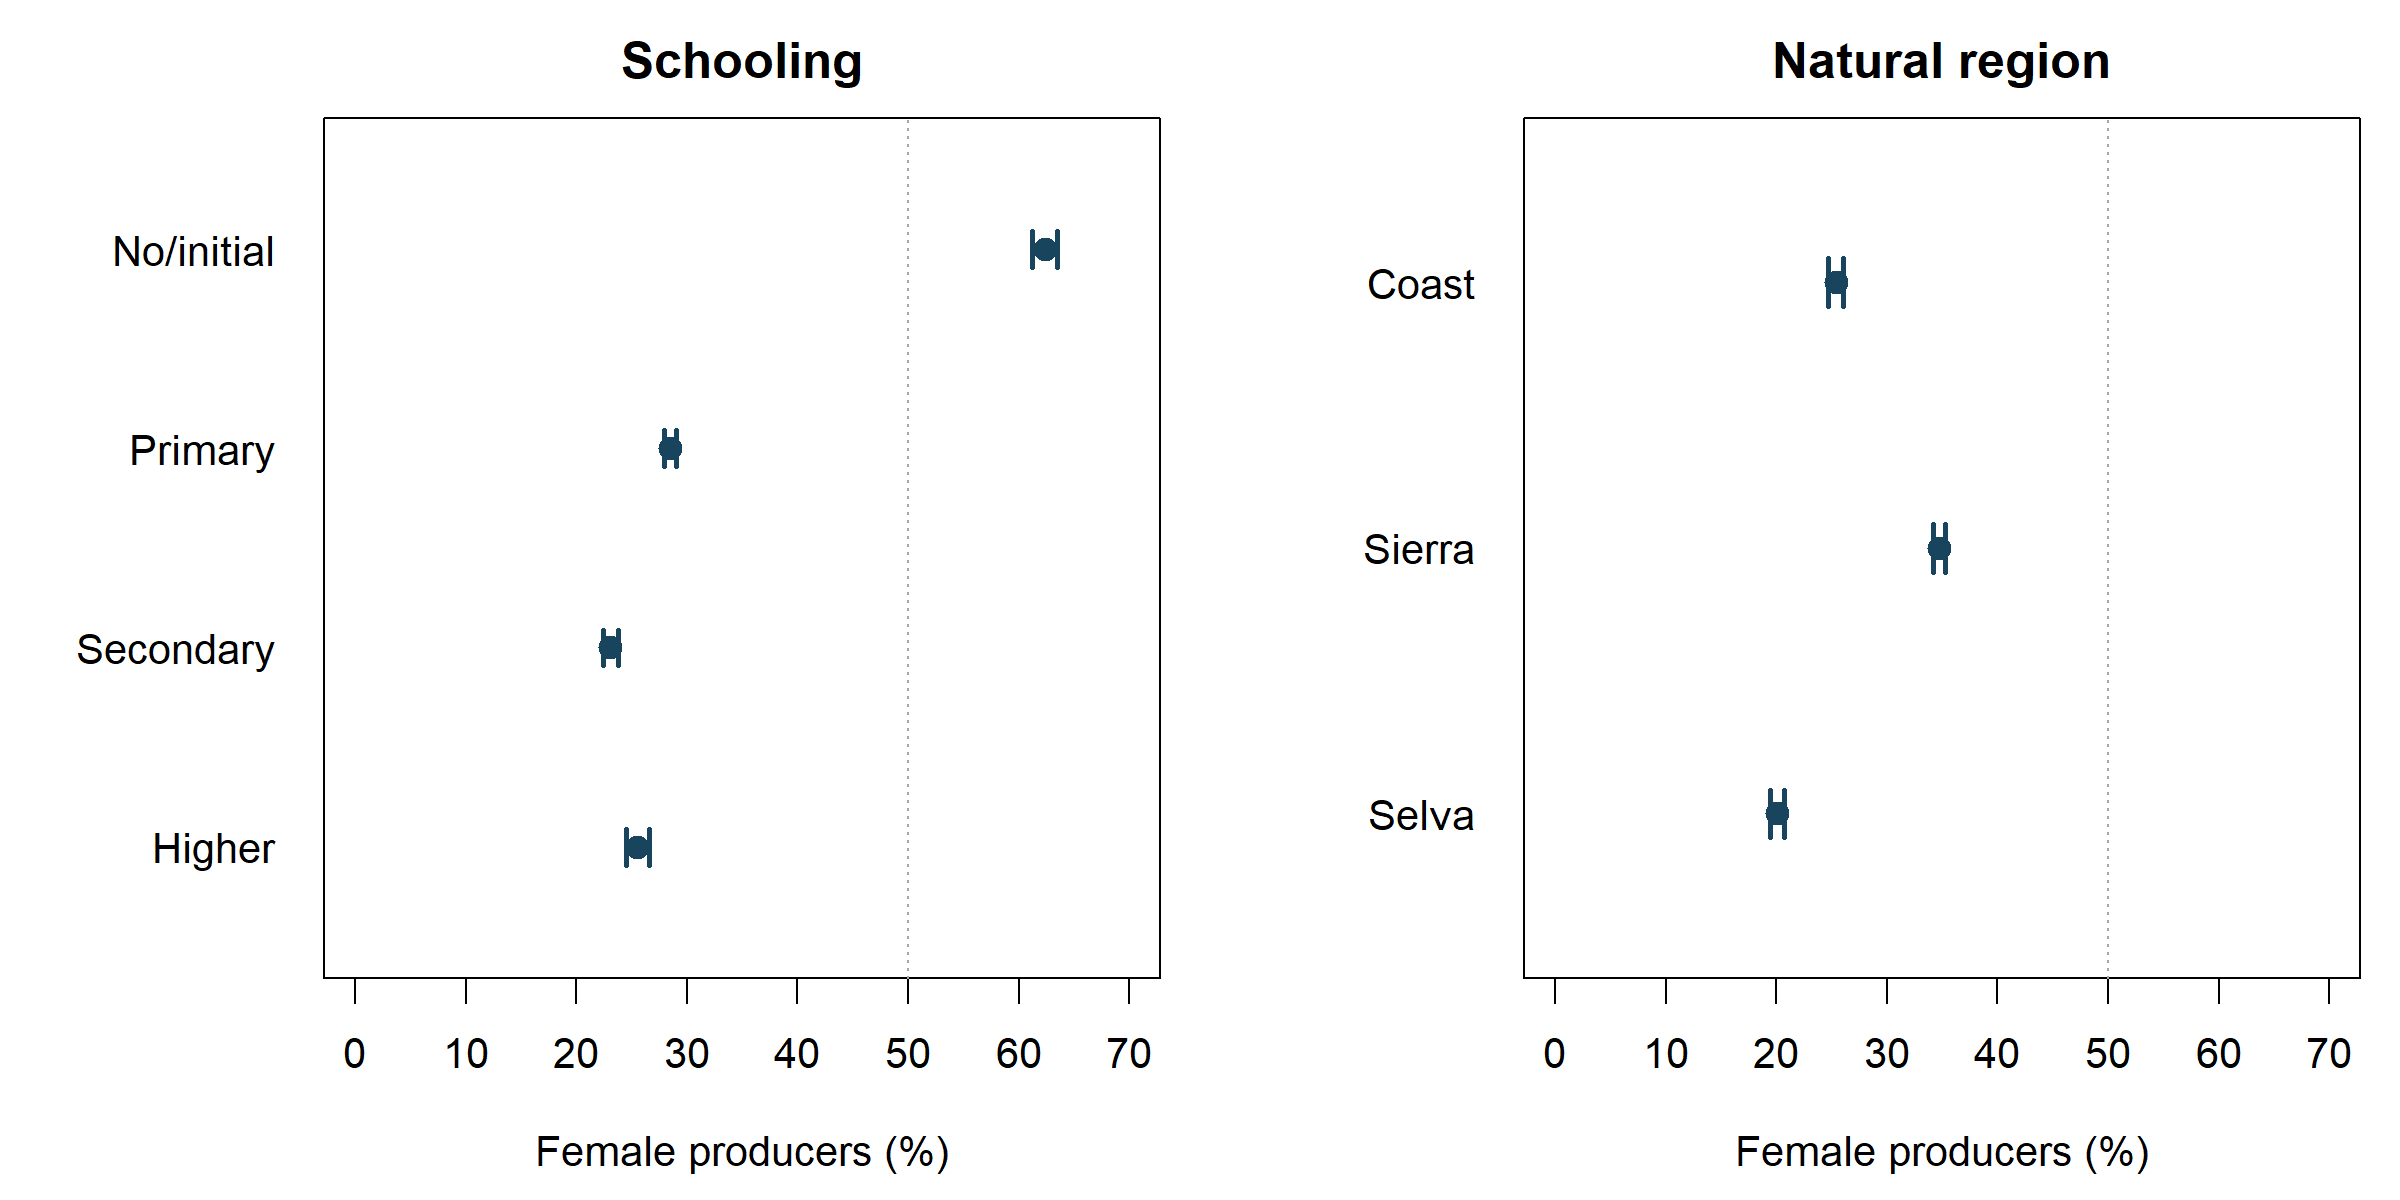
\includegraphics[width=0.98\textwidth]{figure2_subgroup_shares_ci.png}
\caption{Female share within schooling and natural-region groups across pooled producer-rounds. Points are survey-weighted estimates and bars are approximate 95\% confidence intervals under the analytical design. The two panels classify the same records by different variables; group estimates should not be added across panels.}
\label{fig:subgroups}
\end{figure}

\subsection{Adjusted associations and temporal assessment}
After adjustment for age, its quadratic term, natural region, and round, every schooling category had lower female odds than no/initial schooling (Table~\ref{tab:model}). The primary-schooling odds ratio was 0.219 (95\% CI 0.206--0.233), while the Sierra-to-Coast ratio was 1.273 (1.216--1.333). The signs were the same in separate 2014--2022 and 2023--2025 fits, though magnitudes differed. For example, the primary-schooling ratio was 0.204 in the older era and 0.271 in the newer era. This is directional robustness rather than proof that the associations are invariant to redesign.

\begin{table}[htbp]
\centering\small
\caption{Selected survey-weighted logistic associations, pooled and by survey era.}
\label{tab:model}
\begin{tabular}{lccc}
\toprule
Contrast (reference) & Pooled OR (95\% CI) & 2014--2022 OR (95\% CI) & 2023--2025 OR (95\% CI) \\
\midrule
Primary (no/initial) & 0.219 (0.206--0.233) & 0.204 (0.196--0.213) & 0.271 (0.220--0.335) \\
Secondary (no/initial) & 0.151 (0.141--0.162) & 0.141 (0.134--0.148) & 0.186 (0.149--0.232) \\
Higher (no/initial) & 0.176 (0.162--0.192) & 0.177 (0.166--0.187) & 0.190 (0.147--0.244) \\
Sierra (Coast) & 1.273 (1.216--1.333) & 1.245 (1.197--1.294) & 1.339 (1.180--1.520) \\
Selva (Coast) & 0.636 (0.600--0.674) & 0.589 (0.559--0.621) & 0.769 (0.660--0.895) \\
\bottomrule
\end{tabular}
\begin{minipage}{0.96\textwidth}\footnotesize\vspace{2mm}
All models include age, $(\mathrm{age}/10)^2$, and round indicators. Confidence intervals use Taylor linearization under the analytical-strata approximation. OR = odds ratio. Round coefficients are omitted because frame changes preclude a simple temporal interpretation.
\end{minipage}
\end{table}

Standardizing over the weighted 2025 covariate distribution gave a modeled female probability of 66.82\% (approximate 95\% CI 64.32--69.32) if all records were assigned no/initial schooling, compared with 31.26\% (29.23--33.29) if assigned primary schooling. The analogous probabilities were 29.20\% (27.23--31.17) for Coast and 34.16\% (32.05--36.27) for Sierra. These estimates hold the observed 2025 distribution of other modeled covariates fixed; they do not represent the effects of changing a person's education or location. The full set of conditional standardized predictions is supplied with the supplementary analysis.

The separate prediction model trained through 2024 had weighted AUC 0.615 in 2025. Its Brier score was 0.206, compared with 0.215 for the constant-rate training baseline. Mean predicted female probability was 28.61\% while the observed weighted share was 31.18\%, an underprediction of 2.57 percentage points. Figure~\ref{fig:calibration} shows observed and predicted shares across weighted prediction deciles in the 2025 holdout. This split therefore provides limited evidence of transportability and no basis for individual decisions.

\begin{figure}[H]
\centering
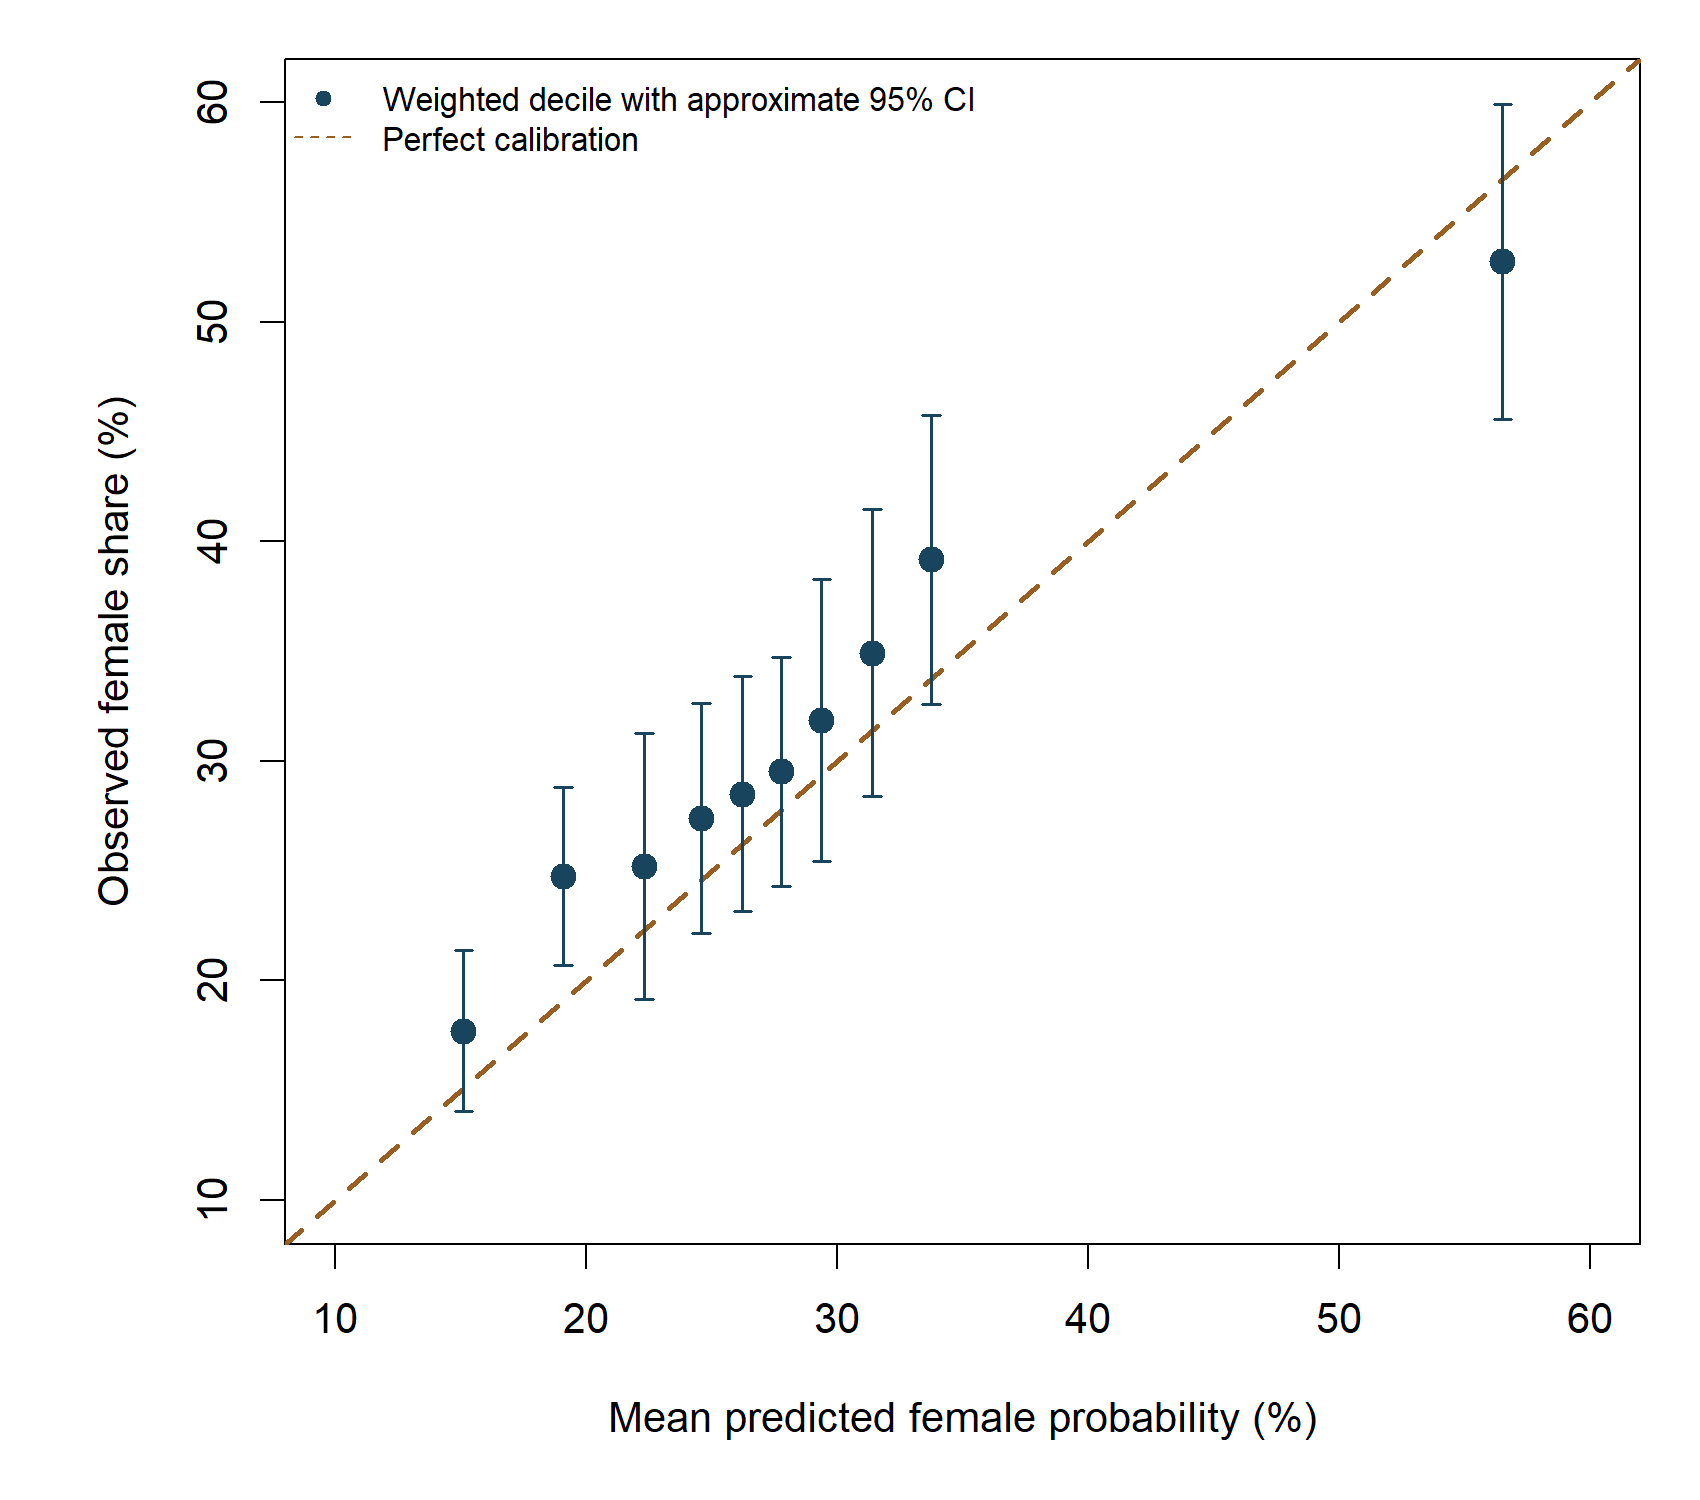
\includegraphics[width=0.68\textwidth]{figure3_2025_calibration.png}
\caption{Calibration of the model trained on rounds through 2024 in the held-out 2025 round. Each point represents approximately one tenth of the 2025 expansion weight, grouped by predicted probability; horizontal position is the weighted mean prediction and vertical position is the observed female share, with an approximate 95\% confidence interval. The dashed diagonal denotes perfect calibration. Decile groups are descriptive and do not replace the overall calibration and discrimination measures.}
\label{fig:calibration}
\end{figure}

\subsection{Access to services and finance in the 2025 round}
The 2025 producer sample included 9,691 female-coded and 28,758 male-coded records. Women represented 31.18\% of the weighted producer population, matching the rounded official estimate of 31.2\% \cite{inei2025results}. Female producers were more often in the Sierra (77.72\% versus 65.56\%), had no or initial schooling more often (14.99\% versus 4.65\%), and operated a smaller median area (2.25 versus 3.55 hectares). These are 2025 descriptions, not changes measured across the full series.

Training was reported by 5.28\% of female and 8.37\% of male producers (raw difference $-3.09$ percentage points, approximate 95\% CI $-5.28$ to $-0.90$). Credit application was reported by 8.37\% and 11.65\%, respectively (difference $-3.28$, $-5.32$ to $-1.24$). The fully adjusted differences were $-2.29$ ($-4.93$ to 0.36) and $-1.27$ ($-3.38$ to 0.85) percentage points, respectively (Table~\ref{tab:access}, Figure~\ref{fig:access}). Technical-assistance and savings-account intervals also included zero. These adjusted contrasts standardize across observed covariates and do not measure the effect of changing sex or allocate a causal share of the raw gaps to any variable.

\clearpage
\begin{table}[H]
\centering\scriptsize
\caption{Service and financial-access outcomes by recorded producer sex in ENA 2025.}
\label{tab:access}
\begin{tabular}{p{2.6cm}rrrr}
\toprule
Outcome & Male, \% & Female, \% & Raw difference, pp (95\% CI) & Adjusted difference, pp (95\% CI) \\
\midrule
Training & 8.37 & 5.28 & $-3.09$ ($-5.28$, $-0.90$) & $-2.29$ ($-4.93$, 0.36) \\
Technical assistance & 3.97 & 3.21 & $-0.77$ ($-2.21$, 0.67) & 0.21 ($-1.41$, 1.82) \\
Credit application & 11.65 & 8.37 & $-3.28$ ($-5.32$, $-1.24$) & $-1.27$ ($-3.38$, 0.85) \\
Savings account & 29.90 & 28.15 & $-1.75$ ($-5.21$, 1.70) & 1.07 ($-2.48$, 4.62) \\
\bottomrule
\end{tabular}
\begin{minipage}{0.96\textwidth}\footnotesize\vspace{2mm}
pp = percentage points. Training and assistance refer to the preceding three years; financial questions to the preceding 12 months. Adjusted differences use sex, age, age squared, schooling, natural region, operated area, and an area-missing indicator. All intervals are approximate under the recorded-stratum design with singleton-stratum adjustment.
\end{minipage}
\end{table}

\begin{figure}[H]
\centering
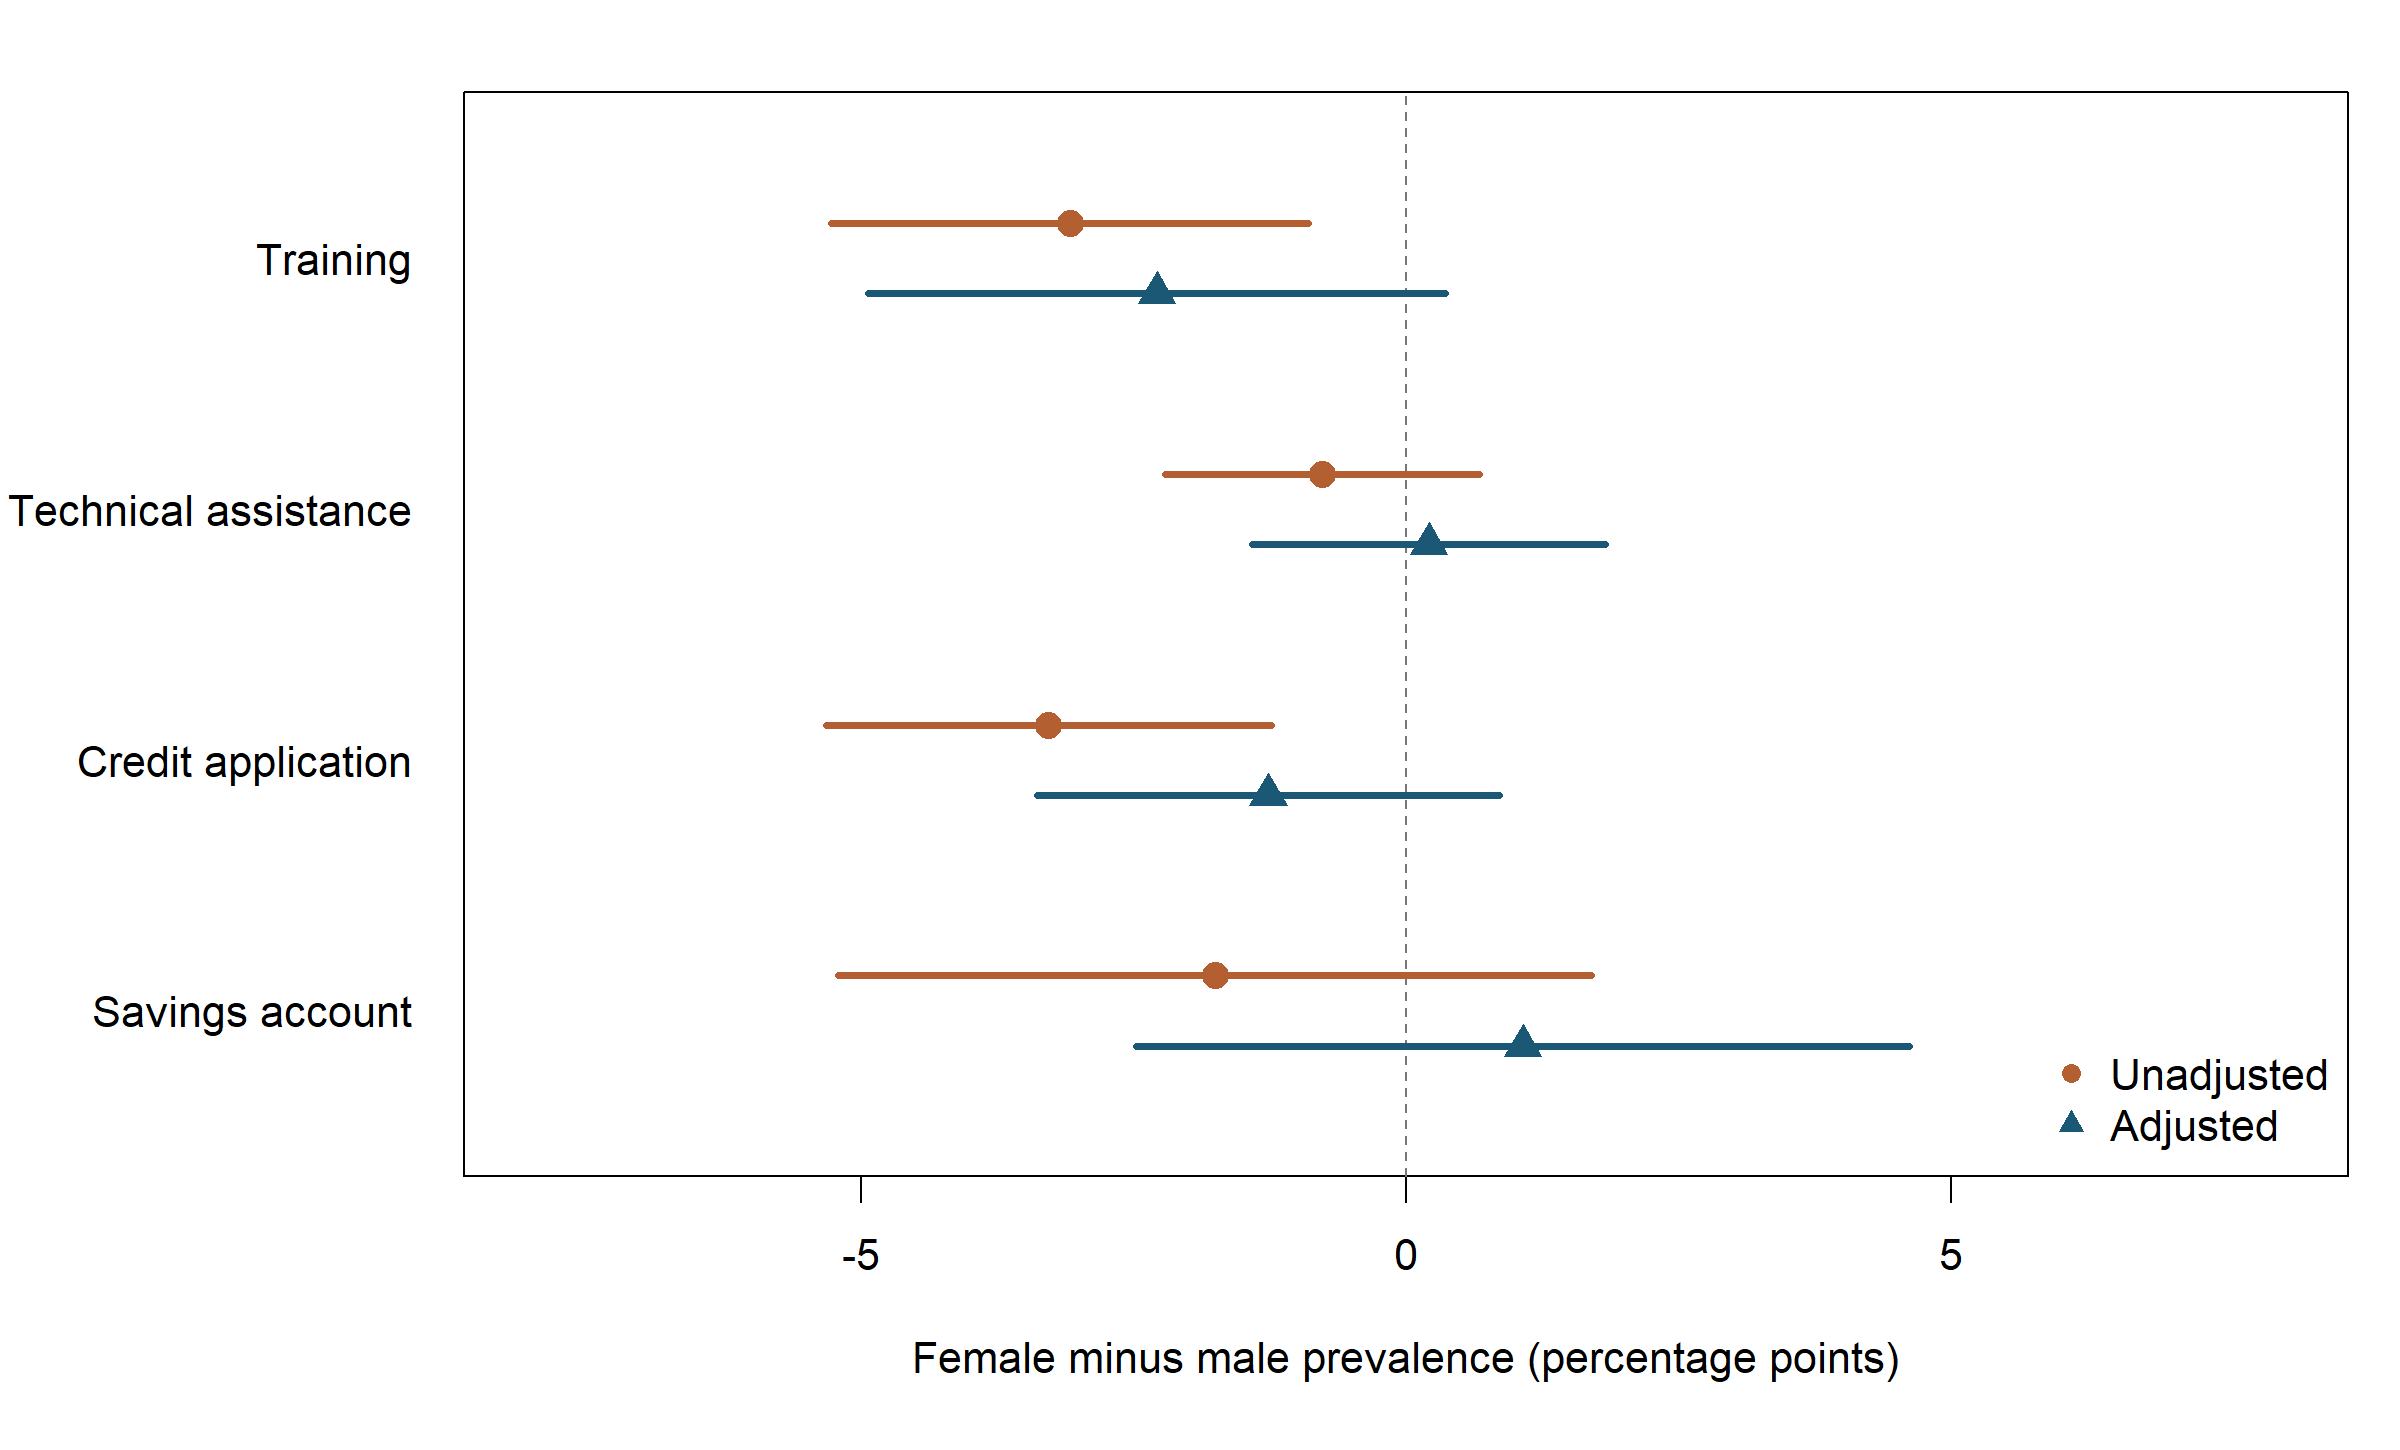
\includegraphics[width=0.92\textwidth]{figure1_access_gaps.png}
\caption{Female-minus-male prevalence differences for four access outcomes in 2025. Points show raw survey estimates and model-standardized differences, with approximate 95\% confidence intervals. The adjusted intervals condition on the observed covariate distribution.}
\label{fig:access}
\end{figure}

Of 4,646 unweighted credit applicants, 3,799 were male and 847 female. The weighted receipt rate among applicants was 94.01\% for men and 87.92\% for women (Figure~\ref{fig:credit}). The adjusted female-to-male odds ratio was 0.39 (approximate 95\% CI 0.18--0.86). It was 0.39 (0.17--0.89) with department fixed effects and 0.39 (0.19--0.81) when using department as the analytical stratum. The crude odds-ratio interval included 1. Application is a selected stage, and unmeasured collateral, loan amount, lender, and creditworthiness prevent a discrimination inference.

\begin{figure}[H]
\centering
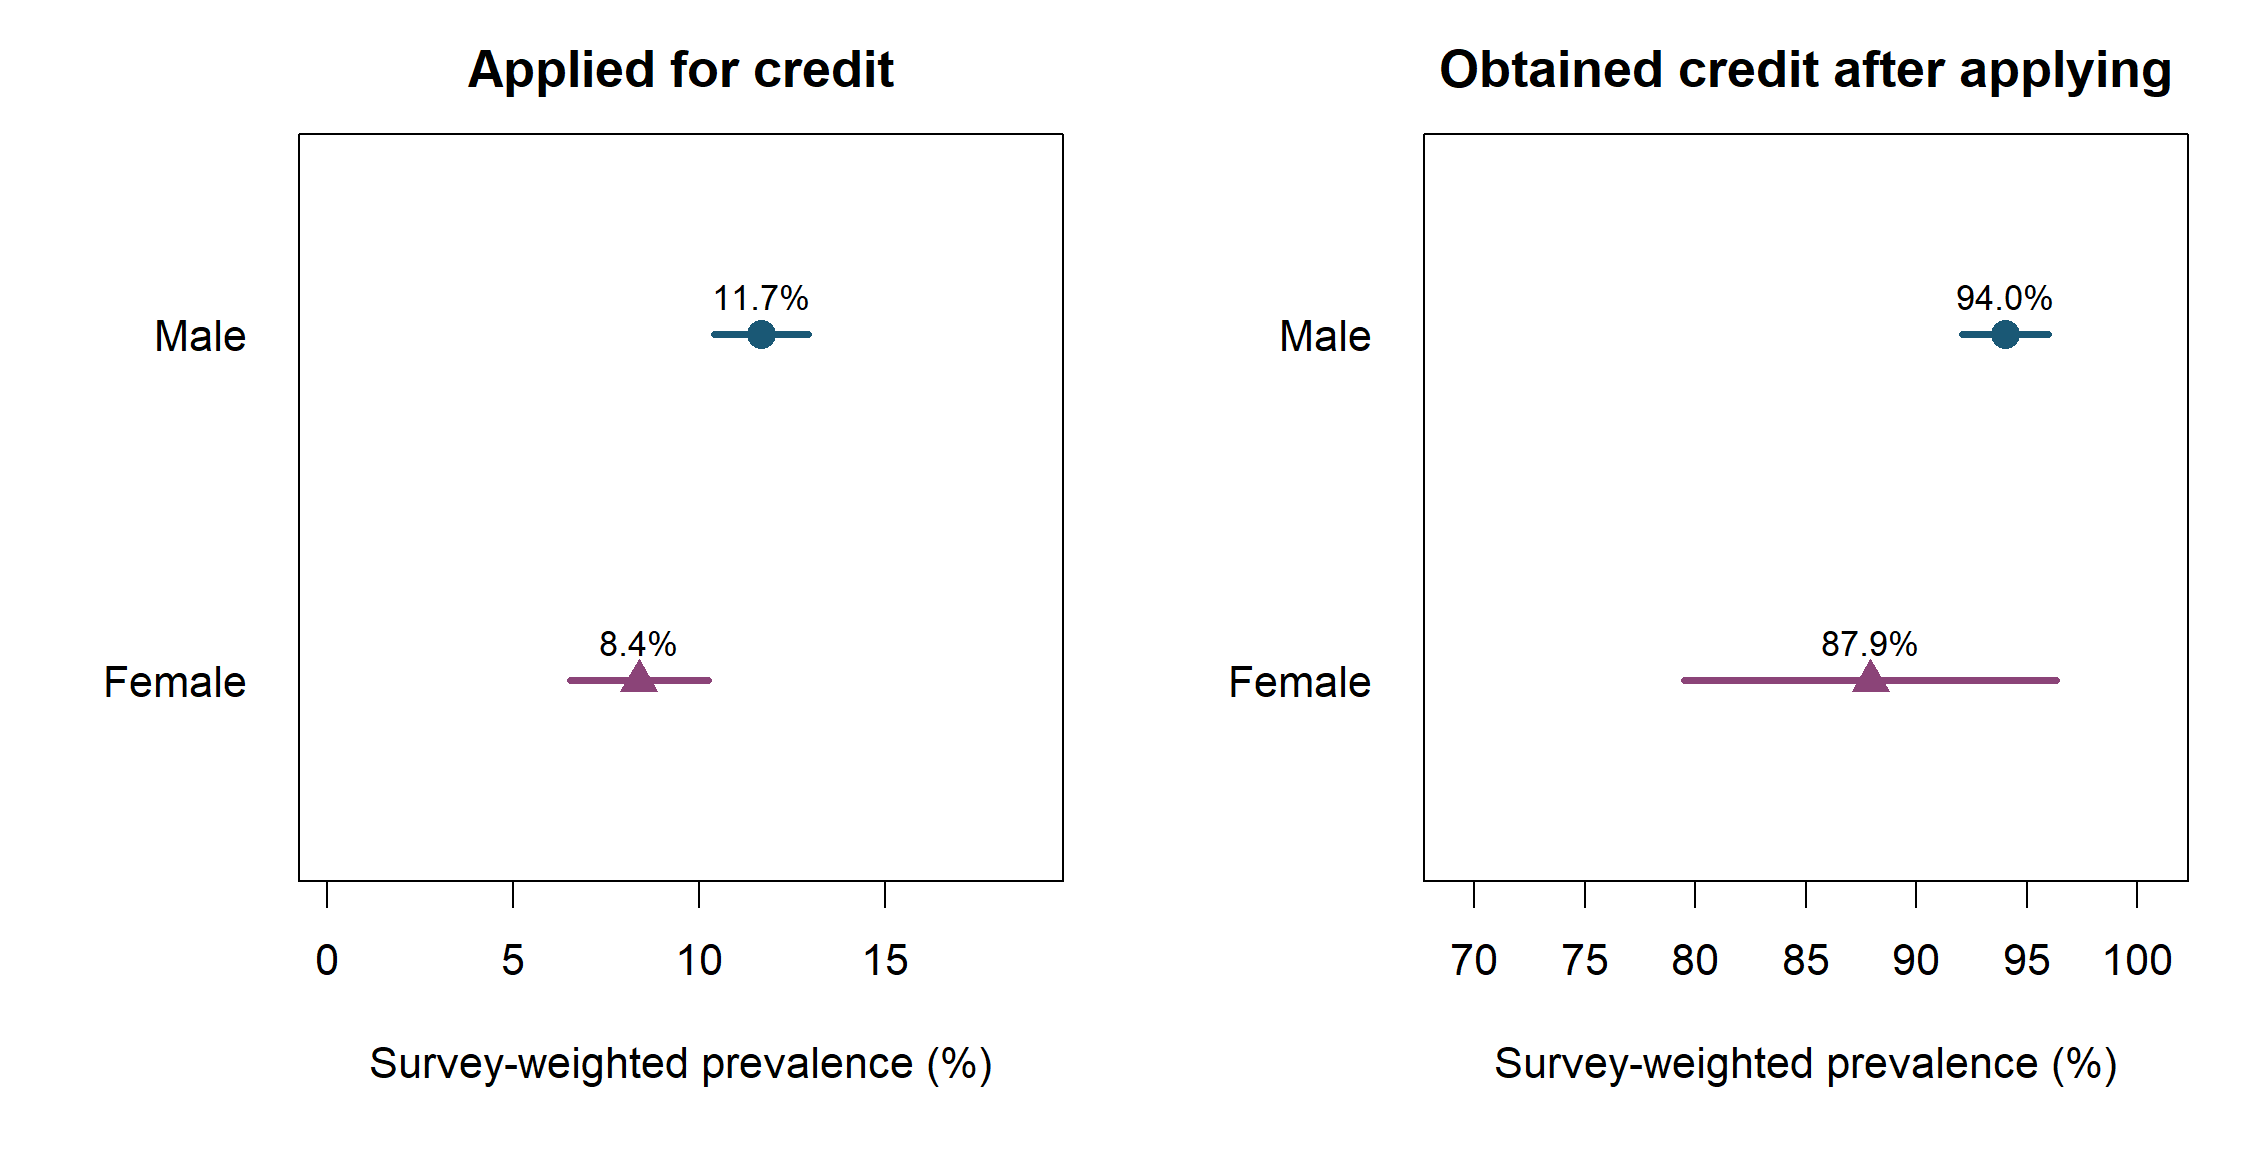
\includegraphics[width=0.82\textwidth]{figure3_credit_stages.png}
\caption{Two distinct credit denominators in 2025. The left panel shows application among all producers; the right shows receipt of requested credit among applicants. Points are survey-weighted percentages with approximate 95\% confidence intervals. Horizontal scales differ across panels.}
\label{fig:credit}
\end{figure}

\section{Discussion}
The ENA records a larger share of female producers in 2025 than in 2014, with a peak in 2022. More defensible than a single trend statement is the finding that female producer status is unevenly distributed across schooling and natural regions and that the directions of these associations persist on either side of the survey redesign. The no/initial-schooling group has a particularly high female share, and Sierra records have a higher female share than Coast records after adjustment for the modeled covariates. The absolute-scale standardized predictions show that the schooling contrast is not merely a feature of odds-ratio scaling. The education pattern may combine cohort composition, selection into recorded producer status, and other unmeasured circumstances; the present analysis cannot separate these explanations.

These findings describe who is recorded as producer, not why. Prior research shows that women's roles in agriculture can coexist with different combinations of work, ownership, bargaining power, and opportunity \cite{deere2005,doss2018,kawarazuka2022,leder2022}. In Peru, evidence on asset gaps in agricultural units \cite{delpozo2016}, heterogeneous experiences among Sierra potato farmers \cite{patel2018}, and the distinct roles of land ownership, joint titles, and household decisions in welfare and agricultural participation \cite{schling2024,wiig2013,tobin2022} cautions against reading a producer-sex share as a direct welfare measure. The INEI also reports registered land-title ownership separately from producer sex \cite{ineiods2025}; the two indicators have different denominators and should not be equated. These studies and indicators use different samples and outcomes and therefore do not validate or explain the pooled ENA associations. The eleven-round file does not contain harmonized direct measures of male migration, legal title, credit, plot size, income, language, or decision-making. It cannot distinguish empowerment from necessity, widowhood, inheritance, household reporting conventions, or other mechanisms. The education and regional coefficients should not be used to infer effects of schooling policy or geographic relocation.

The 2025 extension and finance modules add a separate, more direct view of opportunity at the endpoint of the series. Lower raw training and credit-application rates among female producers attenuated after adjustment for observed age, schooling, region, and area; the fully adjusted intervals span zero. This does not show that those characteristics caused the gaps, especially because area may itself reflect unequal resources. The conditional credit-receipt association deserves further investigation, but the analysis is restricted to applicants and lacks lending criteria. Existing Peruvian studies have examined how extension and credit relate to production or farm performance using different outcomes and populations \cite{neves2021,rituay2026}; they cannot identify the mechanism behind this 2025 applicant contrast. Nor can a 2025 access snapshot establish how services changed from 2014 to 2025.

Several design and data limits matter for interpretation. First, annual survey targets changed, most visibly around 2023; an endpoint contrast does not identify a secular change in a stable population. The 2025 area frame also excludes peasant and Indigenous communities, whose agricultural roles and land governance merit separate study \cite{inei2025,sarapura2022}. Second, historical official stratum variables were not fully preserved. The working round-by-department strata permit transparent approximate intervals, but their precision should not be mistaken for official ENA precision. The separate 2025 recorded-stratum analysis has 3,412 singleton strata and also relies on an explicit variance adjustment. Third, a partial panel in 2019 and possible repeated units in adjacent rounds may create dependence unaccounted for in the pooled variance approximation. Fourth, the historical SPSS file was delivered already consolidated; a script that recreates it from all separate annual modules was not supplied. Fifth, variables that could confound the schooling, regional, service, and applicant comparisons, including farm assets, household composition, and lender criteria, could not be harmonized or observed. Sixth, the modest 2025 discrimination and calibration gap show that the fitted sex-status model does not translate into a strong forecast. These limitations constrain the present evidence rather than invalidate its descriptive patterns.

Future research should harmonize the official annual source modules, document unit and design identifiers across rounds, and examine whether comparable measures of land rights, assets, migration, and agricultural decision-making can be linked. A study designed around those variables could then test mechanisms behind recorded female producer status. Established multidimensional measures such as the Women's Empowerment in Agriculture Index and its project-level version illustrate the additional domains needed to study agency directly \cite{alkire2013,malapit2019}. In the meantime, program evaluation should measure women's access to services and control over resources directly, rather than use a producer-sex share as a proxy for welfare or autonomy.

\section{Conclusion}
In eleven ENA rounds from 2014 to 2025, female producer status was associated with lower schooling categories and Sierra residence. The associations had the same directions in separate older and newer survey eras, while a 2025 holdout showed limited predictive performance. In the 2025 round, female-coded producers reported less training and fewer credit applications than male-coded producers, with uncertain fully adjusted differences. The series and the 2025 access snapshot address different questions. Neither establishes the causes of women's agricultural work, empowerment, or service gaps.

\section*{Data and code availability}
The project repository is available on \href{https://github.com/rntvargas/Gendered-Agricultural-Headship-in-Peru-2014-2025}{GitHub}. The versioned replication snapshot is archived at \url{https://doi.org/10.5281/zenodo.24395430}. These materials contain code, aggregate outputs, source-file hashes, and documentation, without person-level microdata. An earlier historical version has DOI \url{https://doi.org/10.5281/zenodo.24375170}. Official ENA microdata and questionnaires are available from the INEI Microdata Portal \cite{ineiportal}. The project-supplied 2014--2024 consolidated SPSS input and its original construction recipe are not in the public archive; full reproduction from separate historical modules requires that provenance step.

\section*{Ethics statement}
The study reanalyses secondary survey files without contacting participants or reporting individual records. The authors must confirm the institutional ethics determination and complete affiliations, contributions, funding, and competing-interest statements before journal submission.

\begin{thebibliography}{40}\small
\bibitem{alkire2013} Alkire, S., Meinzen-Dick, R., Peterman, A., Quisumbing, A. R., Seymour, G., and Vaz, A. (2013). The Women's Empowerment in Agriculture Index. \emph{World Development}, 52, 71--91. \url{https://doi.org/10.1016/j.worlddev.2013.06.007}
\bibitem{deereleon2003} Deere, C. D., and Le\'on, M. (2003). The gender asset gap: Land in Latin America. \emph{World Development}, 31(6), 925--947. \url{https://doi.org/10.1016/S0305-750X(03)00046-9}
\bibitem{deere2005} Deere, C. D. (2005). \emph{The feminization of agriculture? Economic restructuring in rural Latin America}. UNRISD Occasional Paper 1. \url{https://digitallibrary.un.org/record/545964}
\bibitem{delpozo2016} Del Pozo, C. (2016). \emph{Brechas de g\'enero en el valor econ\'omico de las unidades agropecuarias en el Per\'u}. Consorcio de Investigaci\'on Econ\'omica y Social. \url{https://cies.org.pe/investigacion/brechas-de-genero-en-el-valor-economico-de-las/}
\bibitem{doss2018} Doss, C., Meinzen-Dick, R., Quisumbing, A. R., and Theis, S. (2018). Women in agriculture: Four myths. \emph{Global Food Security}, 16, 69--74. \url{https://doi.org/10.1016/j.gfs.2017.10.001}
\bibitem{fao2023} FAO (2023). \emph{The status of women in agrifood systems}. Rome: FAO. \url{https://doi.org/10.4060/cc5343en}
\bibitem{ineiportal} INEI. Microdata Portal, Encuesta Nacional Agropecuaria. \url{https://proyectos.inei.gob.pe/microdatos/}
\bibitem{inei2018} INEI (2019). \emph{Principales resultados de la Encuesta Nacional Agropecuaria 2018}, survey-design section. \href{https://www.inei.gob.pe/media/MenuRecursivo/publicaciones_digitales/Est/Lib1697/libro.pdf}{Official report}.
\bibitem{inei2019} INEI (2019). \emph{Manual del Encuestador ENA 2019}, Section 3.6. \href{https://proyectos.inei.gob.pe/iinei/srienaho/Descarga/DocumentosMetodologicos/2019-62/04_MANUAL_DEL_ENCUESTADOR_ENA_2019.pdf}{Official manual}.
\bibitem{inei2022} INEI (2023). \emph{33,4\% de los productores agropecuarios del pa\'is son mujeres}. \href{https://m.inei.gob.pe/prensa/noticias/334-de-los-productores-agropecuarios-del-pais-son-mujeres-14486/}{INEI press release}.
\bibitem{inei2023} INEI (2023). \emph{Manual del Entrevistador ENA 2023}, Section 3.6. \href{https://proyectos.inei.gob.pe/iinei/srienaho/Descarga/DocumentosMetodologicos/2023-62/03_MANUAL_DEL_ENTREVISTADOR_ENA_2023.pdf}{Official manual}.
\bibitem{inei2023results} INEI (2024). \emph{Productores Agropecuarios: Principales Resultados de la ENA, 2018, 2019, 2022 y 2023}, Table 5 (2014--2023 retrospective series). \href{https://proyectos.inei.gob.pe/iinei/srienaho/Descarga/DocumentosMetodologicos/2023-62/05_PUBLICACION_ENA_2023.pdf}{Official report}.
\bibitem{inei2025} INEI (2025). \emph{Encuesta Nacional Agropecuaria 2025: Ficha T\'ecnica}, Section 7.9. \href{https://cdn.www.gob.pe/uploads/document/file/4673570/4304991-ficha-tecnica%282%29.pdf}{Official technical sheet}.
\bibitem{inei2025dict} INEI (2025). \emph{Diccionario de Datos, Cap\'itulo 1100}, ENA 2025, Module 1911. Available through the INEI Microdata Portal.
\bibitem{ineigender2025} INEI (2025). \emph{Per\'u: Brechas de G\'enero, 2025: Avances hacia la igualdad de mujeres y hombres}. \href{https://www.inei.gob.pe/media/MenuRecursivo/publicaciones_digitales/Est/Lib2054/libro.pdf}{Official report}.
\bibitem{ineiods2025} INEI (2025). \emph{Per\'u: Evoluci\'on de los Indicadores de los Objetivos de Desarrollo Sostenible (ODS), 2025}. \href{https://www.inei.gob.pe/media/MenuRecursivo/publicaciones_digitales/Est/Lib2062/libro.pdf}{Official report}.
\bibitem{inei2025results} INEI (2026). \emph{Productores Agropecuarios: Principales Resultados de la ENA, 2022--2025}. \href{https://www.gob.pe/institucion/inei/informes-publicaciones/8259187-productores-agropecuarios-principales-resultados-de-la-encuesta-nacional-agropecuaria-ena-2022-2025}{Official results}.
\bibitem{kabeer1999} Kabeer, N. (1999). Resources, agency, achievements: Reflections on the measurement of women's empowerment. \emph{Development and Change}, 30(3), 435--464. \url{https://doi.org/10.1111/1467-7660.00125}
\bibitem{kawarazuka2022} Kawarazuka, N., Doss, C. R., Farnworth, C. R., and Pyburn, R. (2022). Myths about the feminization of agriculture: Implications for global food security. \emph{Global Food Security}, 33, 100611. \url{https://doi.org/10.1016/j.gfs.2022.100611}
\bibitem{leder2022} Leder, S. (2022). Beyond the feminization of agriculture: Rural out-migration, shifting gender relations and emerging spaces in natural resource management. \emph{Journal of Rural Studies}, 91, 157--169. \url{https://doi.org/10.1016/j.jrurstud.2022.02.009}
\bibitem{lumley2004} Lumley, T. (2004). Analysis of complex survey samples. \emph{Journal of Statistical Software}, 9(8), 1--19. \url{https://doi.org/10.18637/jss.v009.i08}
\bibitem{malapit2019} Malapit, H. J., Quisumbing, A. R., Meinzen-Dick, R., Seymour, G., Martinez, E. M., Heckert, J., Rubin, D., Vaz, A., and Yount, K. M. (2019). Development of the project-level Women's Empowerment in Agriculture Index (pro-WEAI). \emph{World Development}, 122, 675--692. \url{https://doi.org/10.1016/j.worlddev.2019.06.018}
\bibitem{neves2021} Neves, M. C. R., Silva, F. de F., and Freitas, C. O. (2021). \emph{The effect of extension services and credit on agricultural production in Bolivia, Peru, and Colombia}. Inter-American Development Bank. \url{https://doi.org/10.18235/0003404}
\bibitem{oecd2026} OECD (2026). \emph{Policies for the Future of Farming and Food in Peru}. OECD Agriculture and Food Policy Reviews. Paris: OECD Publishing. \url{https://doi.org/10.1787/4a2aa5b8-en}
\bibitem{patel2018} Patel-Campillo, A., and Salas Garc\'ia, V. B. (2018). Un/associated: Accounting for gender difference and farmer heterogeneity among Peruvian Sierra potato small farmers. \emph{Journal of Rural Studies}, 64, 91--102. \url{https://doi.org/10.1016/j.jrurstud.2018.10.005}
\bibitem{rituay2026} Rituay, P., Aldea, C., Otoya-Barrenechea, J., Tolentino Soriano, M. A., Garc\'ia, L., and Campos Trigoso, J.-A. (2026). Agricultural credit, farm performance and technology adoption under credit rationing in Peru. \emph{Sustainability}, 18(6), 2761. \url{https://doi.org/10.3390/su18062761}
\bibitem{sarapura2022} Sarapura-Escobar, S., and Hoddy, E. T. (2022). Safeguarding the land to secure food in the highlands of Peru: The case of Andean peasant producers. \emph{Frontiers in Sustainable Food Systems}, 6, 787600. \url{https://doi.org/10.3389/fsufs.2022.787600}
\bibitem{schling2024} Schling, M., and Pazos, N. (2024). Effective land ownership, female empowerment, and food security: Evidence from Peru. \emph{World Development}, 181, 106680. \url{https://doi.org/10.1016/j.worlddev.2024.106680}
\bibitem{steyerberg2010} Steyerberg, E. W., Vickers, A. J., Cook, N. R., Gerds, T., Gonen, M., Obuchowski, N., Pencina, M. J., and Kattan, M. W. (2010). Assessing the performance of prediction models: A framework for traditional and novel measures. \emph{Epidemiology}, 21(1), 128--138. \url{https://doi.org/10.1097/EDE.0b013e3181c30fb2}
\bibitem{strobe2007} von Elm, E., Altman, D. G., Egger, M., Pocock, S. J., G\o tzsche, P. C., and Vandenbroucke, J. P. (2007). The Strengthening the Reporting of Observational Studies in Epidemiology (STROBE) statement: Guidelines for reporting observational studies. \emph{PLoS Medicine}, 4(10), e296. \url{https://doi.org/10.1371/journal.pmed.0040296}
\bibitem{surveydocs} Lumley, T. \emph{survey package documentation}. \href{https://r-survey.r-forge.r-project.org/survey/html/svydesign.html}{Survey design}; \href{https://r-survey.r-forge.r-project.org/survey/html/surveyoptions.html}{variance options}.
\bibitem{tobin2022} Tobin, D., and Castellanos, P. (2022). Gendered differences in decision-making and participation in value chains: Lessons from the highlands of Peru. \emph{Development in Practice}, 32(4), 492--502. \url{https://doi.org/10.1080/09614524.2021.1937555}
\bibitem{wiig2013} Wiig, H. (2013). Joint titling in rural Peru: Impact on women's participation in household decision-making. \emph{World Development}, 52, 104--119. \url{https://doi.org/10.1016/j.worlddev.2013.06.005}
\end{thebibliography}
\end{document}
